%\newpage
\section{Datamining} \label{sec:datamining}
The first step in the process of data mining is to decide for a fitting algorithmm. Because the best algorithm is not known in advance multiple are tested. For this project this were: K nearest Neighbors, Random Forest, Decision Tree, Support vector machine, logistic regression, XGBoost, and four naïve bayes classifiers based on Bernoulli, complement, gaussian  and multinomial.

These ten classification algorithms will be evaluated to determine which one yields the best results. The quality of an algorithm is determined by two properties. The first criterion is a high recall, in order to avoid possible Type 2 errors (a patient with a heart disease is diagnosed as negative) in the diagnosis. The second criterion is the number of examinations required. The reason for this is that we want our model to be universally used by doctors. We assume that this is especially the case when even simple examinations yield a good diagnosis. This criterion also corresponds to Occam’s razor.

Besides the before mentioned use of scalers, imputers and samplers we additionally apply a variety of classifier specific hyperparameters. For the KNN we added the number of used Neighbors from 2 to 97 moving in 5-unit steps as well as the distance metric L1 and L2 as hyperparameters. Random Forest was tested with 10 to 90 (10-unit steps) estimators and a maximum depth of None, 2, 6 and 10 and a minimum split of 2, 6, and 10. Decisions Trees were tested with both the gini index and entropy as impurity measures while the values for maximum tree depth and minimum split were the same as for Random Forest. In the case of logistic regression, we added the same distance options as for KNN. For SVC we tested C values ranging from 120 to 160 (20-unit steps), in combination with the gamma values 0.0001, 0.001, 0.01 and the kernel options linear, polynomial, sigmoidal and radial basis function. For the four naïve bayes estimators we applied alpha values from 0 to 19.5 (0.5-unit steps).

In order to find the best model a stratified nested cross validation was conducted while using two 10-folds. To later decide which model was the best one a classification report for every outer loop of the cv was saved. To run all cvs the work was split into several small parts where every unique combination of estiamtor, scaler and imputer represents its own part that was run on its own. This leads to 210 seperateseperate cross validations. In the following evaluation only the best cv according to the previously defined criterions (high recall and simplicity) are reviewed in greater detail. For measuring the simplicity the minimum percentage to be dropped was used as a metric. If models performed equally we followed Occams Razor and favoured models with a low number of columns and basic preprocessing. The results for every model can be seen in \cref{table:modelresults} in addition to some further prediction metrics without any ordering.


% INSERT TABLE

\begin{table}[]
	% \begin{adjustwidth}{-3cm}{}

	\begin{footnotesize}
		\begin{tabular}{|l|l|l|l|l|l|l|l|}
			\hline
			\textbf{Classifier} & \textbf{Scaler}  & \textbf{Sampler} & \textbf{Rec.} & \textbf{Rec. Std.} & \textbf{AUC.} & \textbf{F1} & \textbf{MPD} \\ \hline
			Baseline            & none             & none             & 1             & 0                  & 50,00         & 0.71        & 0            \\ \hline
			KNN                 & none             & none             & 0.85          & 0.04               & 76.28         & 0.80        & 0            \\ \hline
			XGB                 & Normalizer       & RUS              & 0.77          & 0.09               & 76.54         & 0.78        & 75           \\ \hline
			Random Forest       & StandardScaler   & none             & 0.84          & 0.09               & 78.40         & 0.81        & 100          \\ \hline
			Decision Tree       & none             & none             & 0.85          & 0.06               & 76.70         & 0.80        & 0            \\ \hline
			SVC                 & PowerTransformer & none             & 0.81          & 0.11               & 77.87         & 0.80        & 20           \\ \hline
			NB (bernoulli)      & StandardScaler   & none             & 0.79          & 0.08               & 76.23         & 0.79        & 8            \\ \hline
			NB (complement)     & MinMaxScaler     & none             & 0.84          & 0.03               & 77.48         & 0.81        & 100          \\ \hline
			NB (gaussian)       & Normalizer       & none             & 0.52          & 0.12               & 70.45         & 0.64        & 20           \\ \hline
			NB (multinomial)    & MinMaxScaler     & none             & 0.79          & 0.06               & 76.46         & 0.79        & 100          \\ \hline
			logistic regression & Normalizer       & none             & 0.84          & 0.07               & 76.02         & 0.80        & 0            \\ \hline
		\end{tabular}

		% \begin{adjustwidth}{+3cm}{}
		\begin{center}
			\centering
			RUS = random under sampler, MPD = minimum percentage to be dropped
		\end{center}
		% \end{adjustwidth}
	\end{footnotesize}
	\caption{Best models for every classification algorithm}
	\label{table:modelresults}

	% \end{adjustwidth}
\end{table}

The Table includes the baseline which performs great on our primary decision criterion the recall. But the model would not be usable in the real world because the doctors would not benefit from the "prediction" as they would need to treat every patient special because of the predicted disease. This is why the table also includes AUC and F1 as comparison. 

For the trained models, great differences can be observed with regard to the recall 

While all models have accuracies between 70\% and 79\%, with small confidence intervals respectively, they show great discrepancies in both the total Type 2 errors and the minimum percentage to be dropped. The model with the lowest Type 2 error is the one with KNN (Type 2 = 70), the one with the highest uses naïve bayes gaussian (Type 2 = 233), which is also the model that shows the lowest average accuracy. A total of three models have a minimum percentage to be dropped of 0\% (only features that do not have missing values are maintained), KNN, decision tree and logistic regression. The models with the highest minimum percentage to be dropped which is 100\% are the ones using the Random Forest, and the naïve bayes models using multinomial and complement.

Based on the different model results and our predefined criterion we argue that the best model for classifying whether somebody has a heart disease or not is the model which uses the decision tree, followed closely by the before discussed KNN model.

The decision tree uses no scaler nor sampler and uses the simple imputer and as an additional hyperparameters the gini index was used as impurity measure, while the maximum tree depth was set to none, with a minimum instances per leaf value of 2. The total depth of the tree is 5. Overall, the decision tree model has an average accuracy of 76.7\% and 73 (14.75\% of people with heart disease) Type 2 errors. Due to the good results in the Type 2 errors, the minimum percentage to be dropped (value of 0) and the small size of the accuracy confidence intervals we find the decision tree model despite not having the highest average accuracy to be the one that fulfills our criterions the best. Furthermore, we believe the decision tree model to be the one which is best or the real live use by doctors and patients due to its simplicity.
In order to view what our best model believes to be important indicators we have visualized the best decision tree model in \cref{fig:DecisionTree}. We only display the tree with depth 3 since we aim at focusing on the main attributes. The root node of the tree is whether the participant had asymptomatic chest pain. The node is then split into people who have asymptomatic chest pain and those who do not. The resulting follow up nodes both use gender as the next split. After that the tree splits according to age. Interestingly one can see from this visualization that older men with asymptomatic chest pain have the highest change to be predicted to have a heart disease. Overall, the model predicts men of all ages and with or without asymptomatic chest pain to have a higher probability of having a heart disease compared to women. The group with the lowest chance of having a heart disease are young women with no asymptomatic chest pain.

\begin{figure}[h]
	\centering
	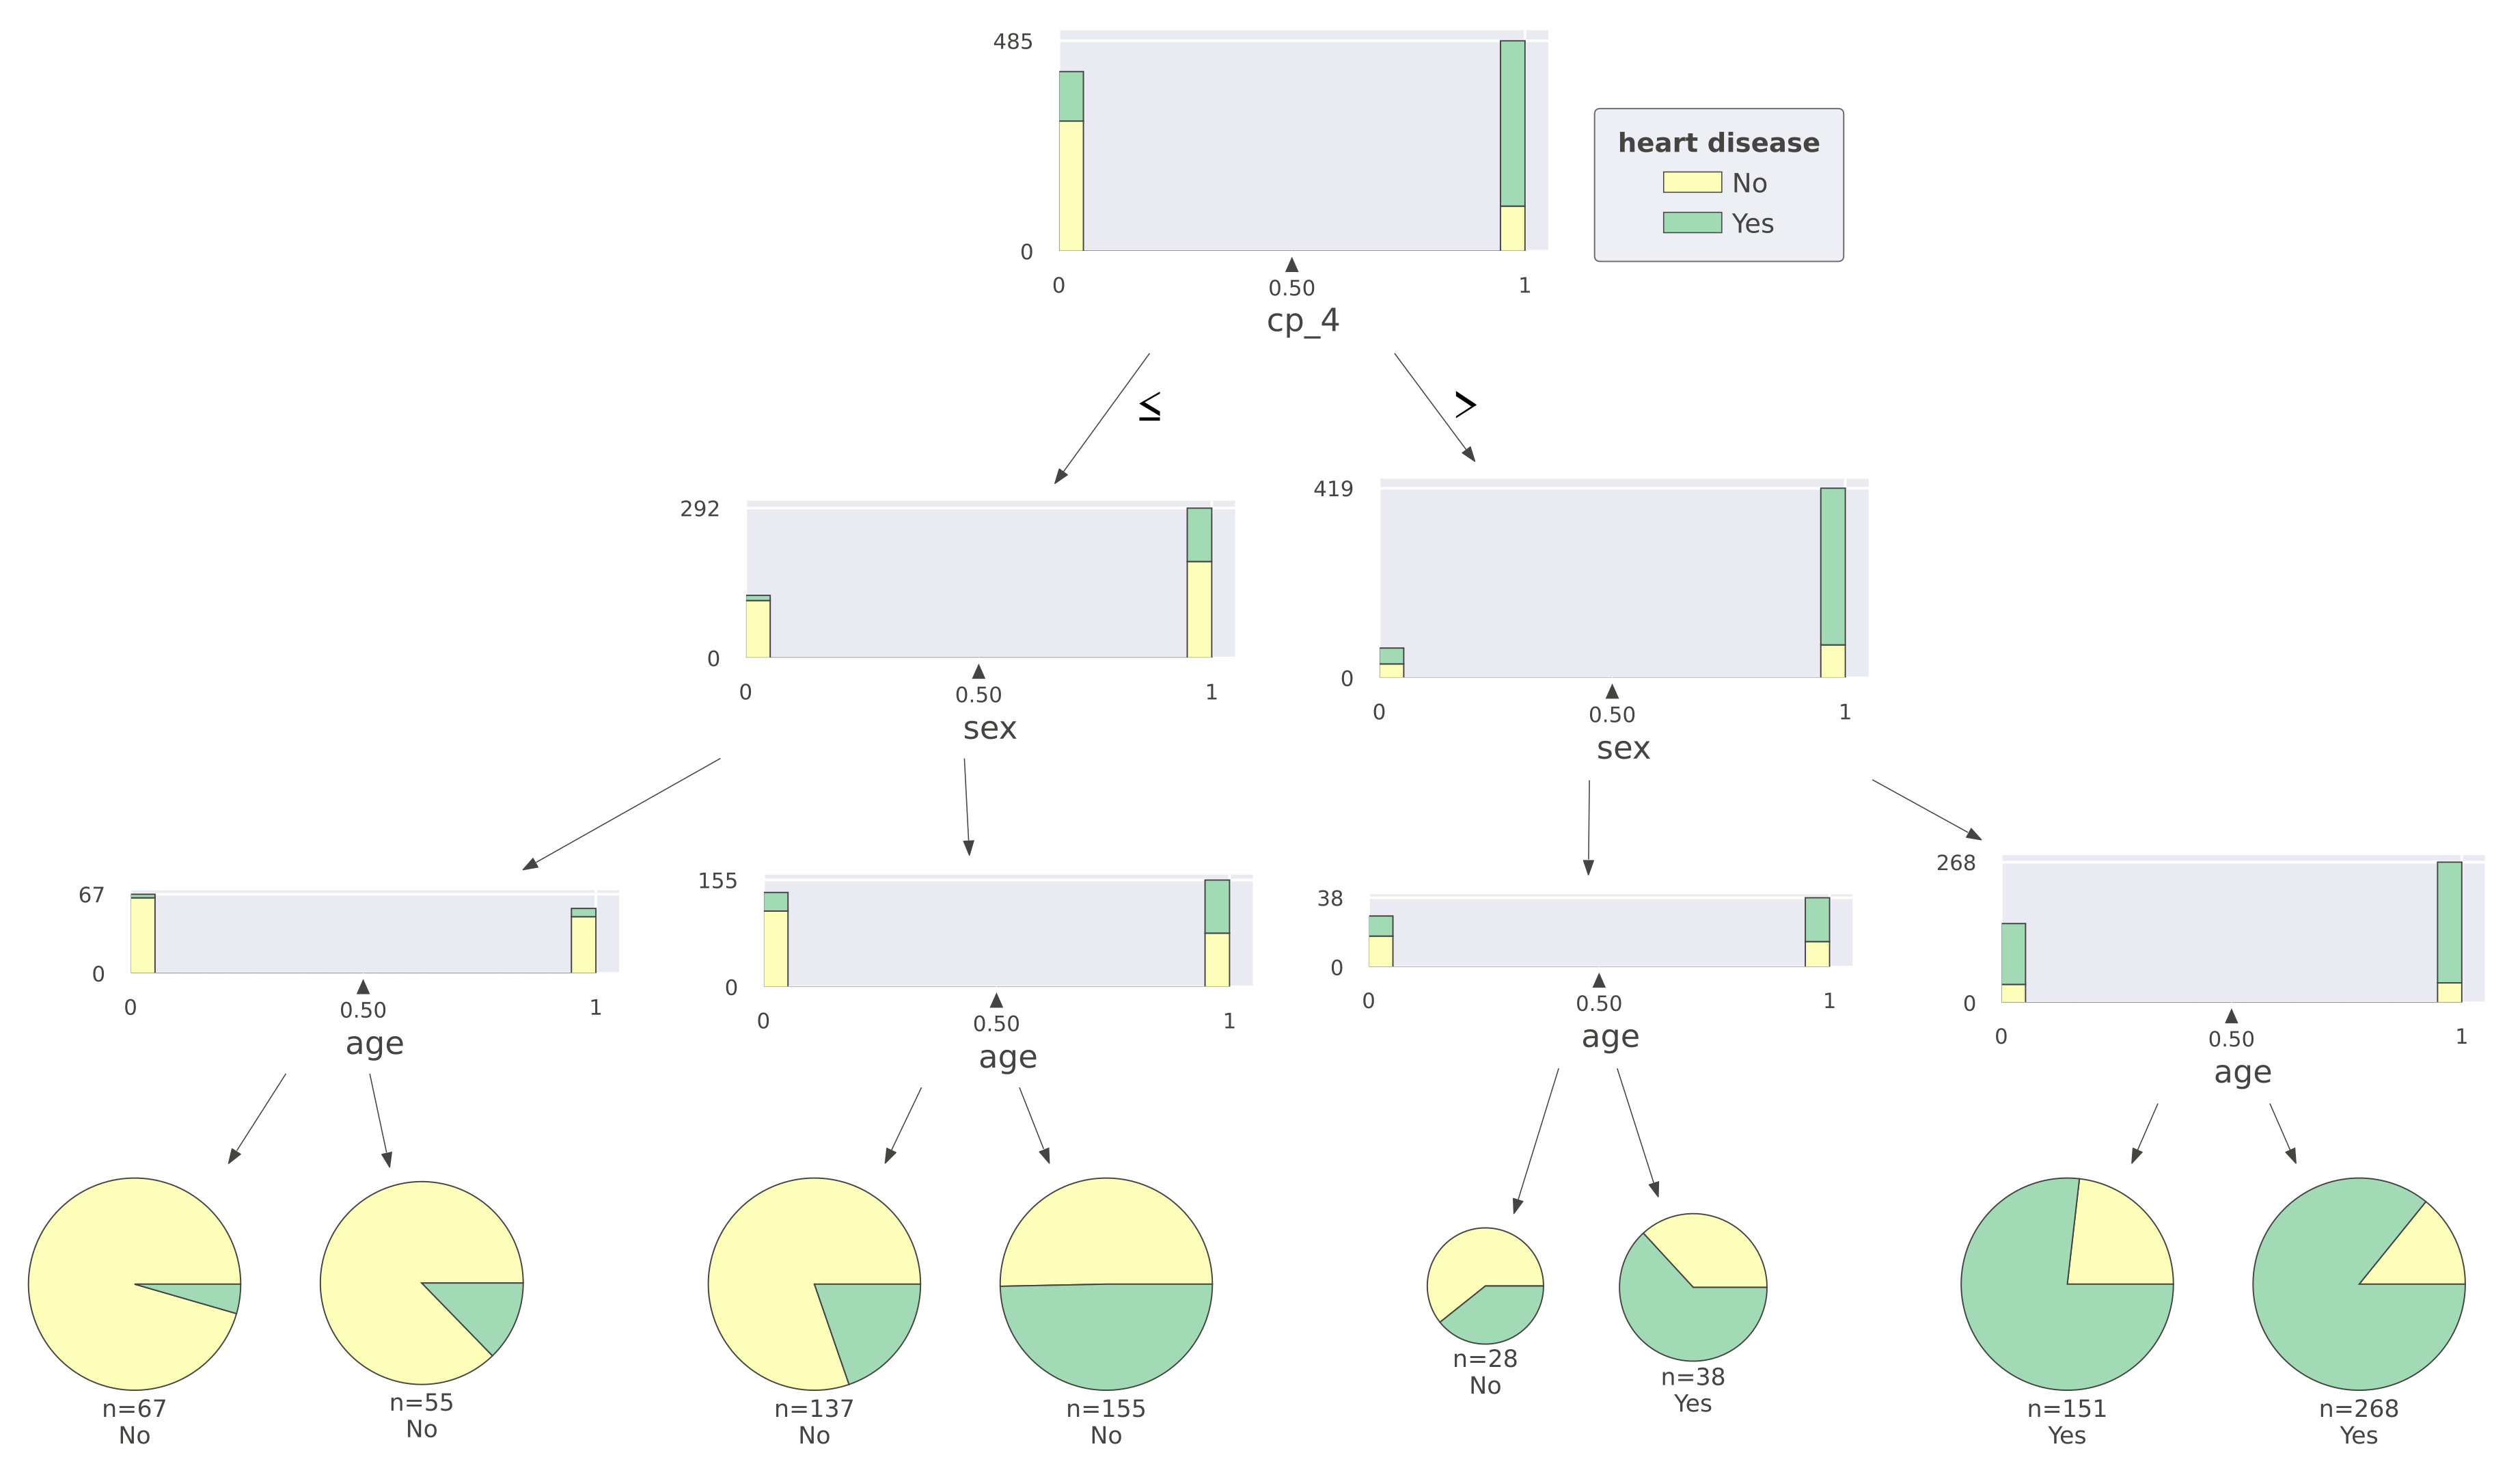
\includegraphics[width=\textwidth]{images/DecisionTree.png}
	\caption{Decision tree visualized}
	\label{fig:DecisionTree}
\end{figure}